\chapter{\IfLanguageName{dutch}{Proof of Concept}{Proof of Concept}}%
\label{ch:PoC}

Dit hoofdstuk biedt een uitgebreid overzicht van een Proof of Concept (PoC) script dat is ontwikkeld voor het lokaal uitvoeren van een Machine Learning pipeline. Het script maakt gebruik van het Prefect-framework voor het orchestreren van de pipelinetaken en MLflow voor het bijhouden van experimenten en logging.

% TODO: verwijs hier naar jouw requirements-analyse waar je bepaalt hebt om Prefect en MLflow te gebruiken

\section{Scenario}

In het opleidingsonderdeel ``Machine Learning Operations'' van de opleiding Toegepaste Informatica kregen studenten een opdracht waarin ze een Machine Learning pipline moesten opzetten met behulp van Azure ML. De studenten dienden een Jupyter notebook te openen die in eerste instantie het model lokaal traint en vervolgens de pipeline opbouwt en doorstuurt naar de Azure. Hierdoor kon de Machine Learning pipeline worden uitgevoerd in de Azure cloud.

Het script bouwt een classificatiemodel om appels van sinaasappels te onderscheiden, bestaande uit drie delen: preprocessing, training en evaluatie. Het preprocessinggedeelte downloadt alle bestanden en herschaalt ze naar een uniforme grootte. Het trainingsgedeelte traint het model, dat bestaat uit verschillende Keras-lagen. Uiteindelijk wordt het model geëvalueerd om de prestaties ervan te meten.

Voor de Proof of Concept van deze bachelorproef wordt hetzelfde script gebruikt zoals in deze opdracht.

\section{Probleemstelling}

% TODO: verwijs hier naar de probleemstelling uit de inleiding. Deze sectie kan je in principe hier ook als basis voor gebruiken!

Om gebruik te kunnen maken van de Azure servers, hebben gebruikers credits nodig. Tijdens de eerder genoemde opdracht waren er studenten die voor aanvang van of tijdens de opdracht geen credits meer hadden. Dit leidde ertoe dat deze studenten hun resultaten niet konden presenteren of zelfs niet konden beginnen aan de opdracht. Daarom wordt in dit onderzoeksvoorstel gekeken naar het opzetten van een lokale installatie van een Machine Learning pipeline.

\section{Uitvoering}

% TODO: ik zou eerst de huidige opstelling van opdracht 3 beschrijven (wat de pipeline doet), evt. met een schematische voorstelling erbij
% TODO: het lijkt alsof de uitleg van Prefect en flow beter in de stand van zaken kan geplaatst worden. Hier kan je dan verwijzen naar de uitleg in de stand van zaken.
% TODO: bouw vervolgens de pipeline stap voor stap op: installatie van de nodige packages (misschien via venv?), preprocessing, training, evaluatie... en maak hiervoor aparte secties

De Proof of Concept zal worden uitgevoerd met behulp van het Prefect-framework samen met MLFlow. Prefect voldoet aan alle criteria van de risicoanalyse en heeft een niet al te steile leercurve, waardoor het een geschikte keuze is voor een labo binnen het opleidingsonderdeel ``Machine Learning Operations''.

Prefect biedt verschillende voordelen ten opzichte van andere frameworks. Ten eerste maakt het eenvoudig plannen van de pipeline mogelijk, zodat deze op een specifiek tijdstip kan worden uitgevoerd. Bovendien is Prefect een Python-bibliotheek, waardoor de enige vereiste kennis Python is, wat mag worden verwacht van de studenten. Daarnaast is het mogelijk om zelf een Prefect server te starten, waardoor alles lokaal kan worden uitgevoerd, wat overeenkomt met het doel van deze proof of concept.

MLFlow zal ook worden gebruikt in deze Proof of Concept. Deze bibliotheek zal zorgen voor het bijhouden van metingen tijdens het machine learning proces. Dit omvat onder andere metingen zoals de nauwkeurigheid van het model, het verlies van het model, en het zal ook alle systeemeigenschappen bijhouden.

Prefect werkt met behulp van ``decorators'', die Prefect in staat stellen om Python-functies te herkennen en uit te voeren als een pipeline. De twee decorators die Prefect gebruikt zijn @task en @flow.

% De @task decorator markeert een functie als een taak, waardoor meerdere taken kunnen worden samengevoegd in een stroom (flow) en in een specifieke volgorde kunnen worden uitgevoerd. Een voorbeeld van een taak in Prefect wordt hieronder gegeven:
% \begin{minted}[frame=lines,breaklines, linenos]{python}
%     @task
%     def my_task():
%         print("Hallo")
% \end{minted}

% In dit voorbeeld zal de taak ``Hallo'' uitprinten en de naam van de functie dient ook als de naam van de taak.

% De @flow decorator combineert alle taken en voert ze vervolgens uit. Een voorbeeld van een flow in Prefect wordt hieronder gegeven:
% \begin{minted}[frame=lines,breaklines, linenos]{python}
%     @flow(name="Test Flow")
%     def main():
%         my_task()
% \end{minted}
In dit voorbeeld zal de flow de taak uitvoeren die eerder is gedefinieerd in een taak. Deze keer wordt een naam aan de flow gegeven, hoewel dit niet strikt noodzakelijk is, kan het helpen om de code overzichtelijker te maken. Er is geen maximumaantal taken dat aan een flow kan worden toegevoegd. Let op dat een taak niet zelfstandig kan worden uitgevoerd deze moet altijd binnen een flow worden geplaatst om te worden uitgevoerd.

De task en flows zijn de core van Prefect. Om te beginnen aan het PoC moet eerst alle nodige Python-biblitheken worden geinstalleer.
De biblitheken die werden gebruikt voor deze PoC zijn:
% \begin{itemize}
%     \item keras (versie 2.15.0)
%     \item mlflow (versie 2.11.3)
%     \item Requests (versie 2.31.0)
%     \item tensorflow (versie 2.15.0)
% \end{itemize}

% deze kunnen als volgt worden geinstalleerd: 

% \begin{minted}{text}
%     pip install keras==2.15.0 mlflow==2.11.3 requests==2.31.0
%     tensorflow==2.15.0 tensorflow_macos==2.15.0
% \end{minted}

Dit PoC is gebaseerd op de notebook van labo 3 in het opleidingsonderdeel ``Machine Learning Operations''
%github?

% \begin{figure}[h]
%     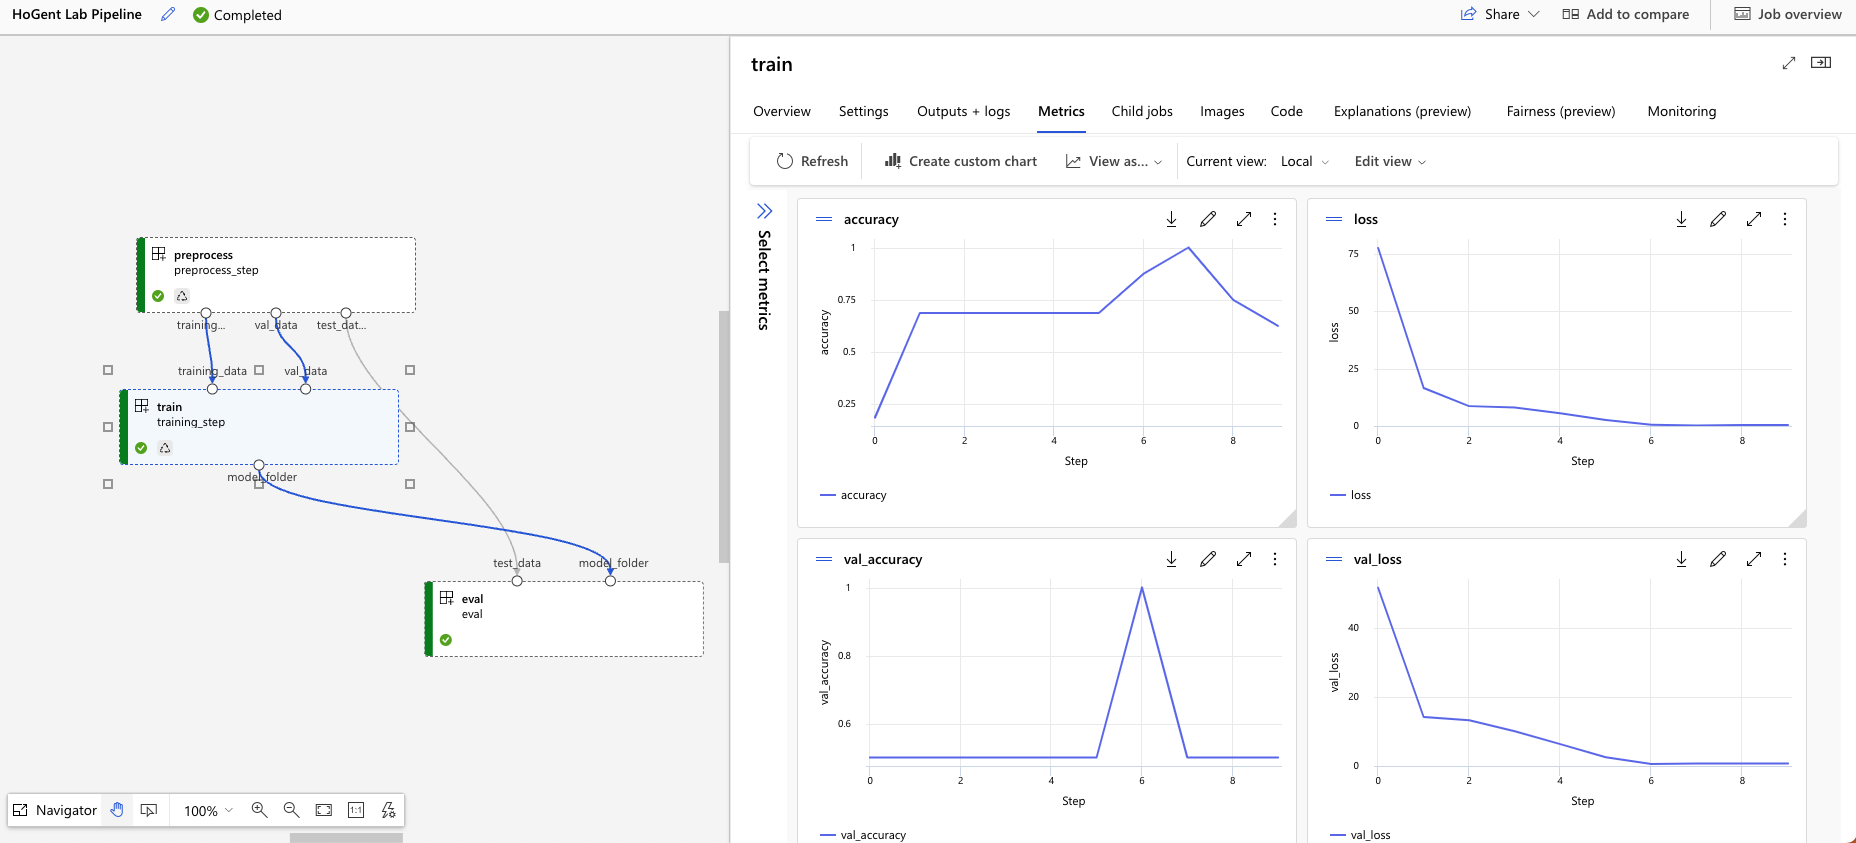
\includegraphics[width=\linewidth]{download.png}
%     \caption{Flow in Azure, Bron: Machine Learning Operations}
%     \label{fig:Resultaten in Azure}
% \end{figure}

%Figuur \ref{fig:Resultaten in Azure} toont de flow aan hoe de notebook van Machine Learning Operations eruit ziet in een Azure omgeving, hier kan duidelijk gezien worden dat er een flow is van 3 taken.
Dit werd eerder toegewezen in het scenario, maar hier zie je de 3 taken: preprocessing, train en eval.

In dit deel van het PoC gaan we het resultaat van labo 3 nabootsen met Prefect.
Om hier aan te beginnen moeten we eerst het orginele notebook omzetten naar Prefect taken en flows. Er zal gefocust worden op de 3 taken preprocessing, train en eval.


